
We measured the performance of PHASTA-chef~\cite{phastachef_github}
POSIX file and data stream information exchange in a workflow supporting
the adaptive analysis of a two-phase, incompressible dam-break flow, as shown in
Fig.~\ref{fig:dambreak}.
Workflow tests ran on the Intel Knights Landing Theta Cray XC40 system at
the Argonne Leadership Computing Facility (ALCF) using 64 processes per node
with a total of 2Ki, 4Ki, 8Ki, and 16Ki processes.
All nodes were configured in the `cache-quad' mode~\cite{knl,jeffers2016intel}.
The two Theta filesystems used by POSIX file tests,
GPFS~\cite{gpfs_2002} and Lustre~\cite{understanding_lustre_2009},
were in their default configuration for all runs.
Test time is recorded using the low-overhead Read Time-Stamp Counter instruction
(\texttt{rdtsc()}) provided by the Intel compiler.
Unlike, some other high resolution timers, \texttt{rdtsc()} is not affected by
variations to the Knights Landing core frequency~\cite{jeffers2016intel}.

Each test initially loads the same mesh with 2Ki parts and 124 million elements.
For the tests running on 4Ki, 8Ki, or 16Ki processes the first step is to
partition the mesh using a graph-base partitioner to the target number of
processes.
Once partitioned, the chef preprocessor is executed.
The preprocessor reads the solution field produced by PHASTA, balances the mesh
using ParMA~\cite{SmithParma2015}, and then creates and writes the PHASTA mesh
and field data structures.
Following the initial preprocessing, the test executes seven
solve-then-preprocess cycles.
In the adaptive workflow used to study the dam-break flow (shown in
Fig.~\ref{fig:dambreak}) the preprocess step is preceded by execution of
MeshAdapt.
For our information exchange performance tests though, this step is not
necessary.
Since we are not adapting the mesh, the mesh size does not change during the
test.
Combining this preprocess-only approach with a limited PHASTA flow
solver execution mode, we can force the workflow to perform the same work in
each cycle.

After preprocessing with chef, the workflow executes the PHASTA
solver.
It starts by reading the mesh and field structures produced by chef
then executes one time step with field updates disabled.
With the field updates disabled the time spent in the solver is the same
in each cycle.
While this configuration does not produce meaningful flow results, it performs
sufficient linear system solve work to emulate the data access and movement of
multiple complete solution steps.
Once the linear system is solved PHASTA writes the solution field and
control passes back to chef to run the preprocessor.
After six more solve-then-preprocess cycles, the test is complete.

The minimum, maximum, and average number of bytes read and written per process
in a cycle by chef and PHASTA is plotted in
Fig.~\ref{fig:totalBytes}.
Since we have a fixed mesh, the bytes read/written at each cycle is the same.
This extends across the different I/O method tests (streams, POSIX,
ramdisk) as the initial partitioning and load balancing called during
preprocessing is deterministic.
Note, in the tested configuration PHASTA writes additional fields that are not
required for input.
Due to the lack of these additional fields the chef byte count is smaller for
write (compared to read), while the PHASTA byte count is smaller for read
(compared to write).

\begin{figure} \centering
  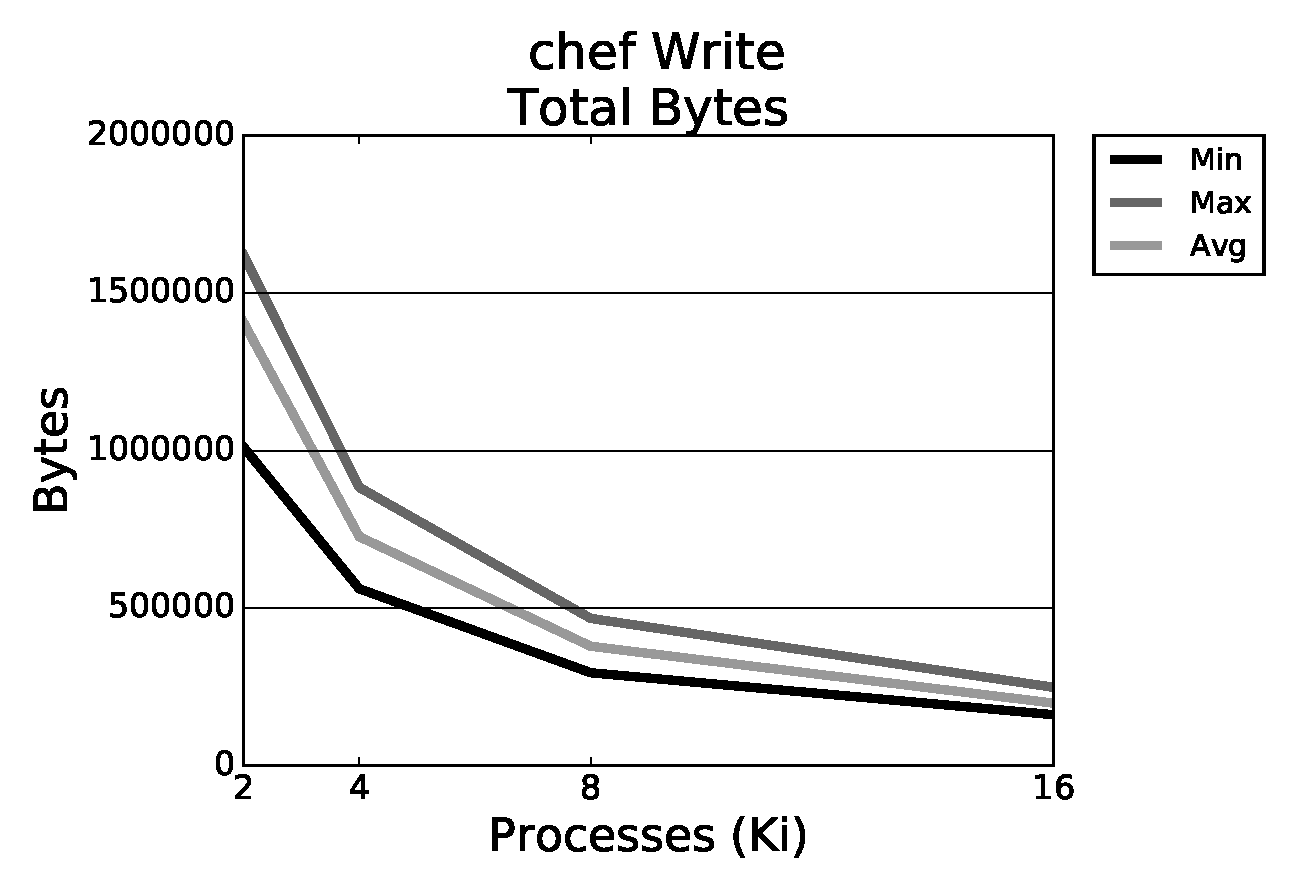
\includegraphics[width=.49\textwidth]{results/phasta-dambreak/theta/streamchefWriteTotalBytes.eps}
  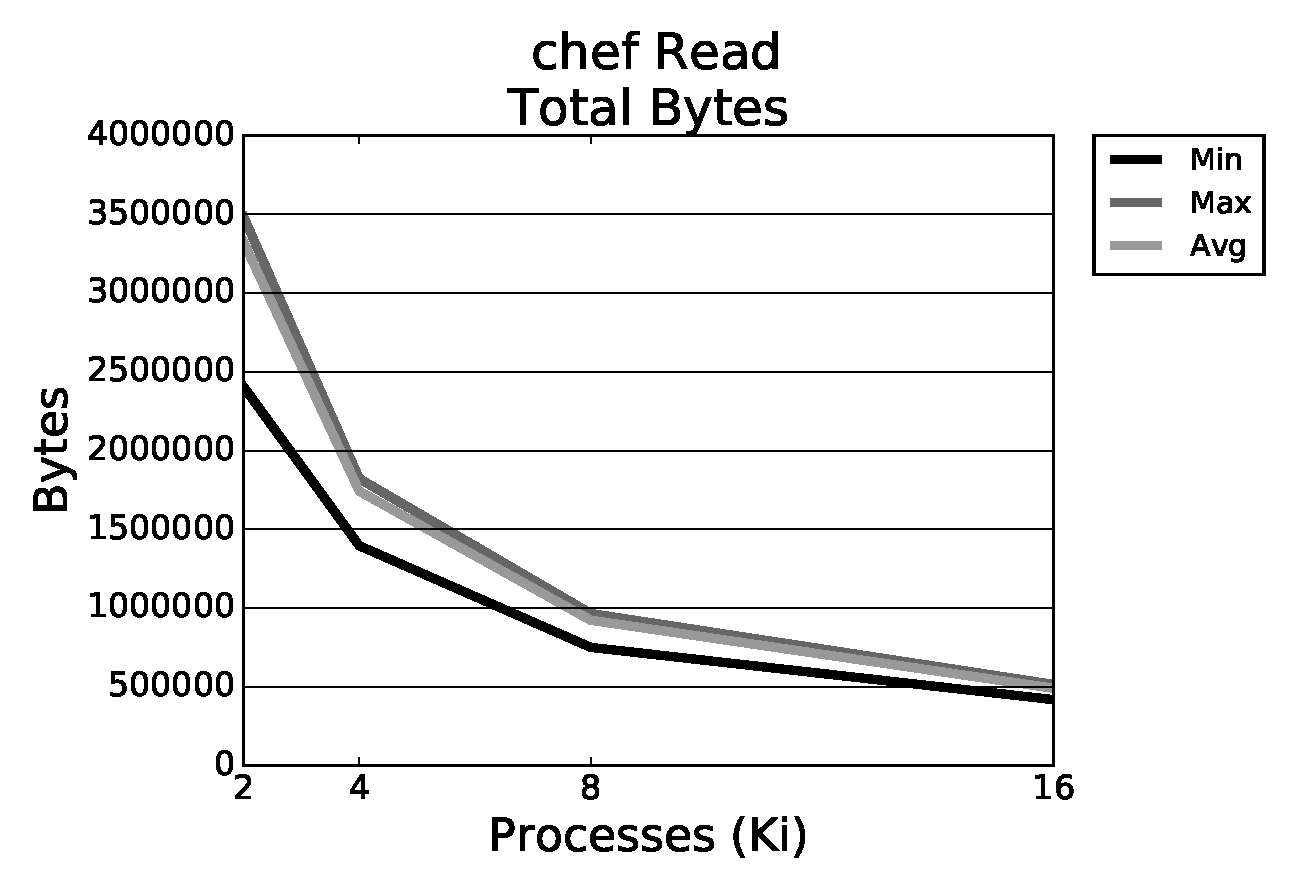
\includegraphics[width=.49\textwidth]{results/phasta-dambreak/theta/streamchefReadTotalBytes.eps}
  \caption{
    chef total bytes read and written per process. PHASTA reads(writes) the same number of
    bytes that chef wrote(reads).
  }
  \label{fig:totalBytes}
\end{figure}

While it may be tempting to report the impact of I/O on the overall workflow
execution time, we omit this statistic as it is highly dependent on the
application and the time it spends in the flow solver and adaptation procedures.
First, the fraction of time spent in I/O decreases as the number of flow solver
steps run between each adaptation increases.
Second, if the implicit solve were replaced by an explicit solve, then the solve
time may decrease by an order of magnitude.
Finally, the number of entities modified or created during adaptation strongly
impacts the fraction of time spent adapting the mesh.
Indeed, prior to this work, the large time spent reading and writing files drove
research towards less frequent adaptation to amortize the I/O time.
The dramatic reduction of time in data transfer provides alternatives.
For these reasons, we choose to primarily report the performance of the
approaches in terms of direct time spent transferring data between components.

The time spent by chef transferring data to and from PHASTA is
reported in Fig.~\ref{fig:readWriteTime} and Fig.~\ref{fig:cheftimes}.
Note, the PHASTA times for these transfers are nearly identical and
not reported here.
Fig.~\ref{fig:readWriteTime} depicts the average time spent reading and writing
at each process count using data streams, a 96GB ramdisk in main memory (DRAM),
and the GPFS and Lustre filesystems.
At each process count Fig.~\ref{fig:chefread} and Fig.~\ref{fig:chefwrite} depict
the time spent reading and writing in each solve-preprocess cycle.
The read time is reported for the function responsible for opening the
PHASTA file/stream containing solution field data, reading the data,
attaching the data to the mesh, and closing the file/stream.
Likewise, the write time includes the time to open, write, and close, plus the
time to detach the solution data from the mesh.

\begin{figure} \centering
  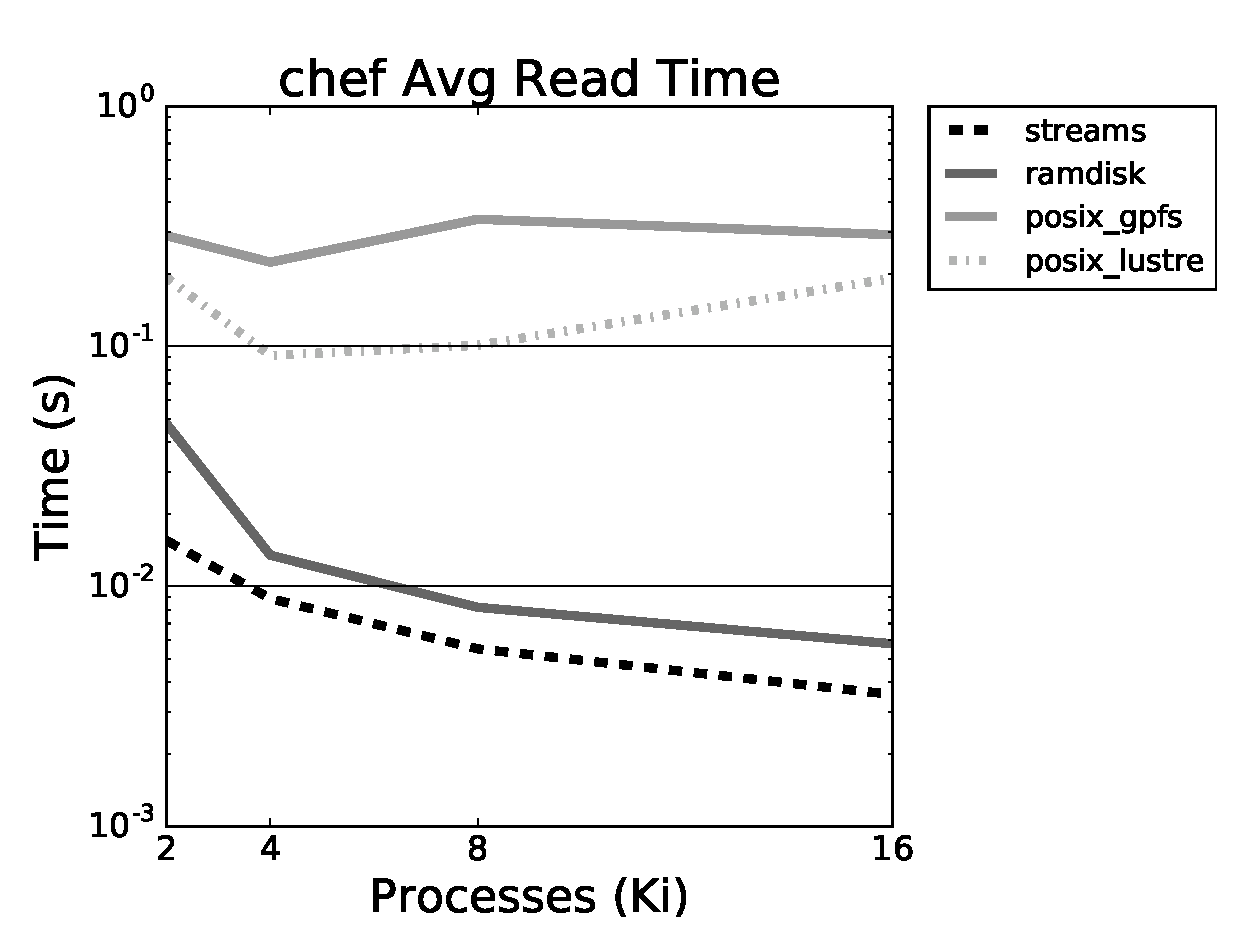
\includegraphics[width=0.49\textwidth]{results/phasta-dambreak/theta/chefreadavg.eps}
  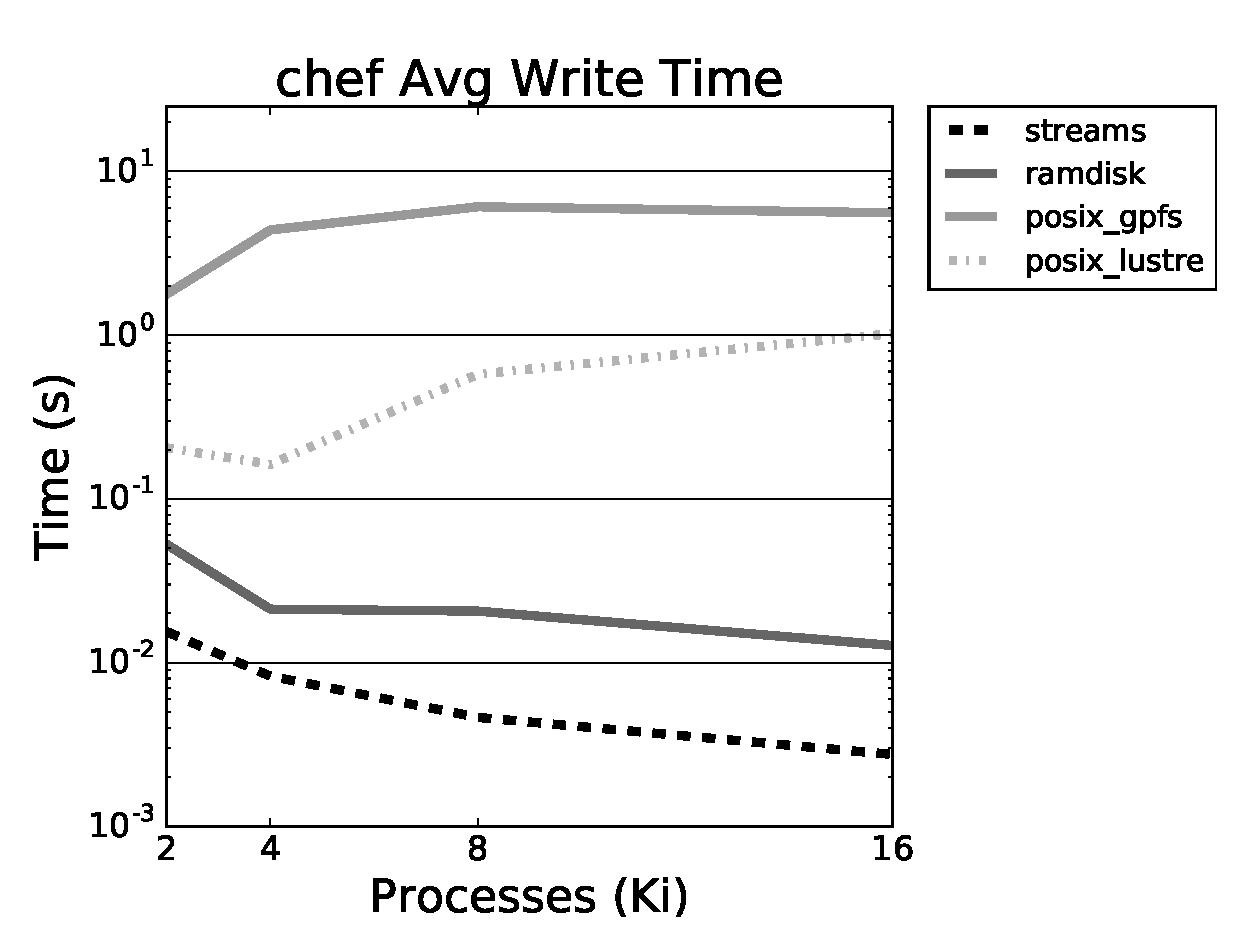
\includegraphics[width=0.49\textwidth]{results/phasta-dambreak/theta/chefwriteavg.eps}
  \caption{
    chef streams, ramdisk, and POSIX average read and write time on
    ALCF Theta. Lower is better.
  }
  \label{fig:readWriteTime}
\end{figure}

\begin{figure} \centering
  \begin{subfigure}{.90\textwidth}
    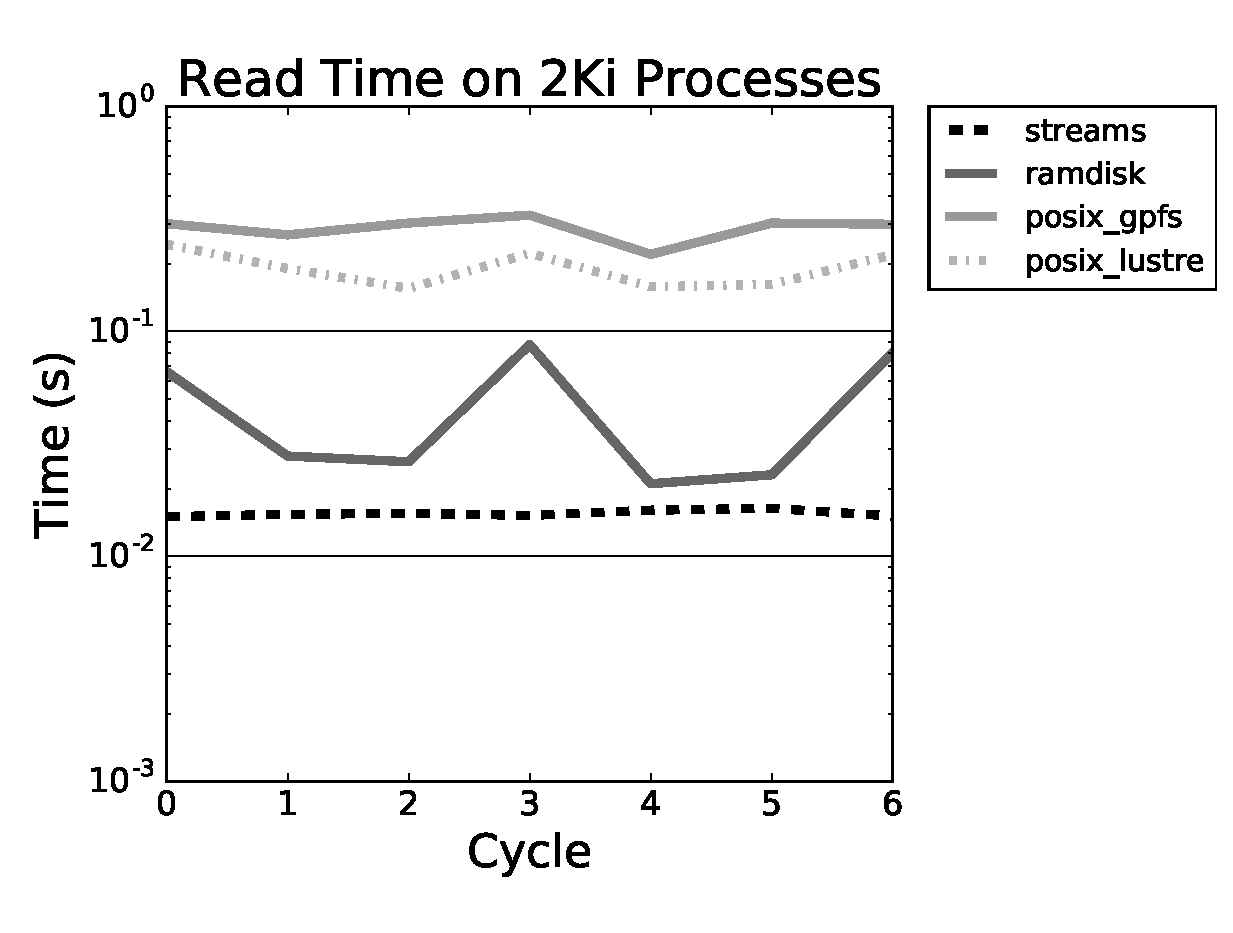
\includegraphics[width=.49\textwidth]{results/phasta-dambreak/theta/chef2048read.eps}
    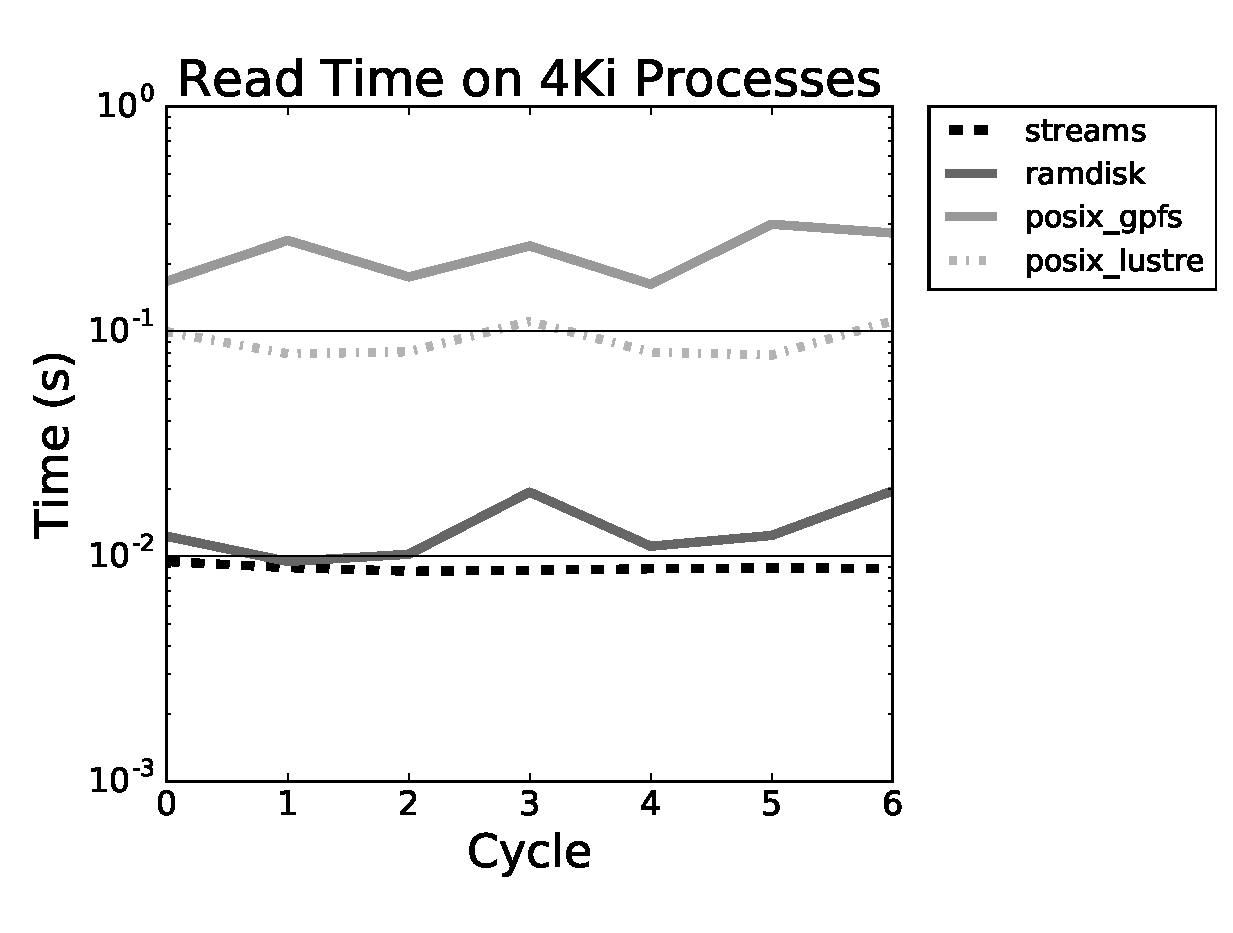
\includegraphics[width=.49\textwidth]{results/phasta-dambreak/theta/chef4096read.eps}
    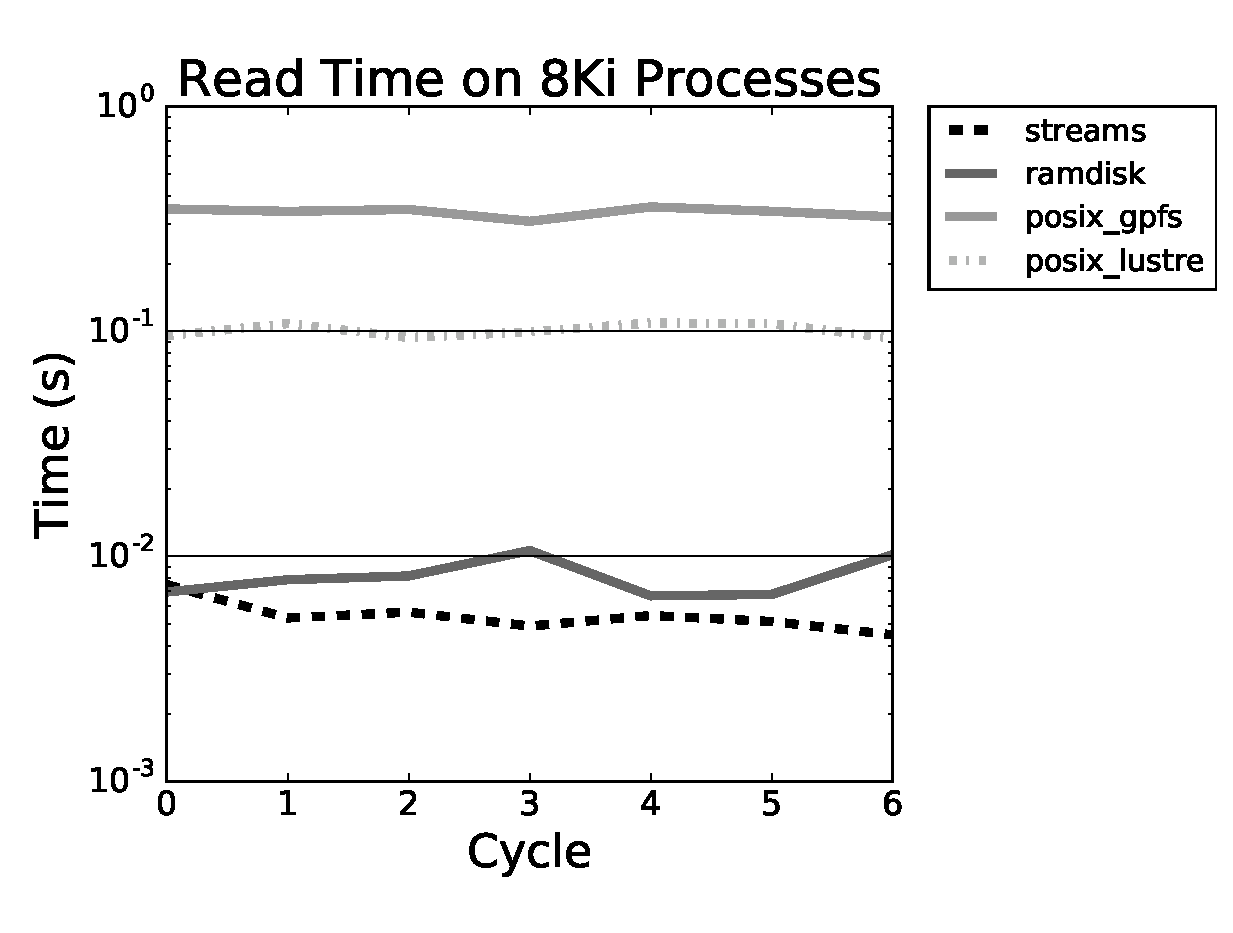
\includegraphics[width=.49\textwidth]{results/phasta-dambreak/theta/chef8192read.eps}
    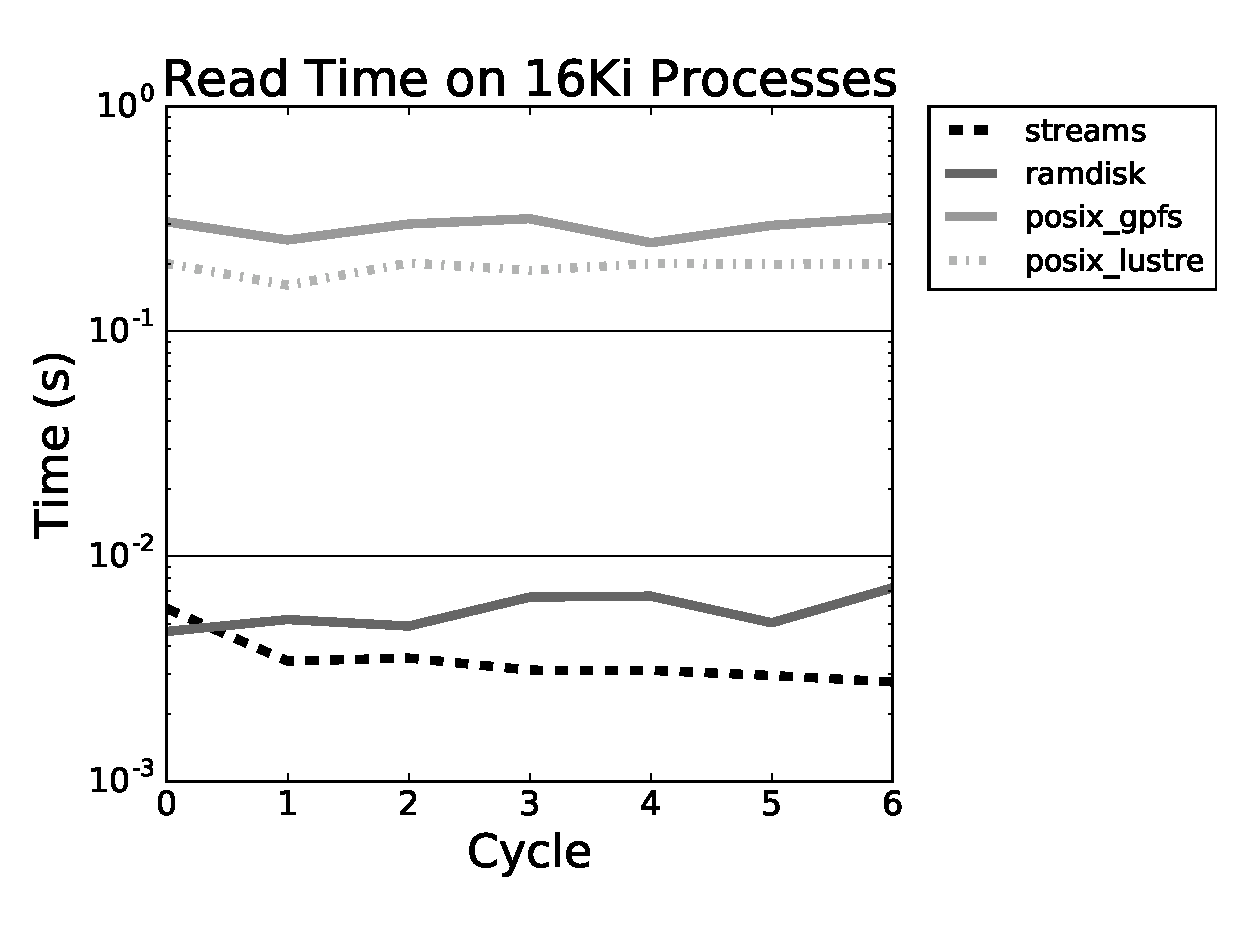
\includegraphics[width=.49\textwidth]{results/phasta-dambreak/theta/chef16384read.eps}
    \caption{chef read times.}
    \label{fig:chefread}
  \end{subfigure}
  \begin{subfigure}{.90\textwidth}
    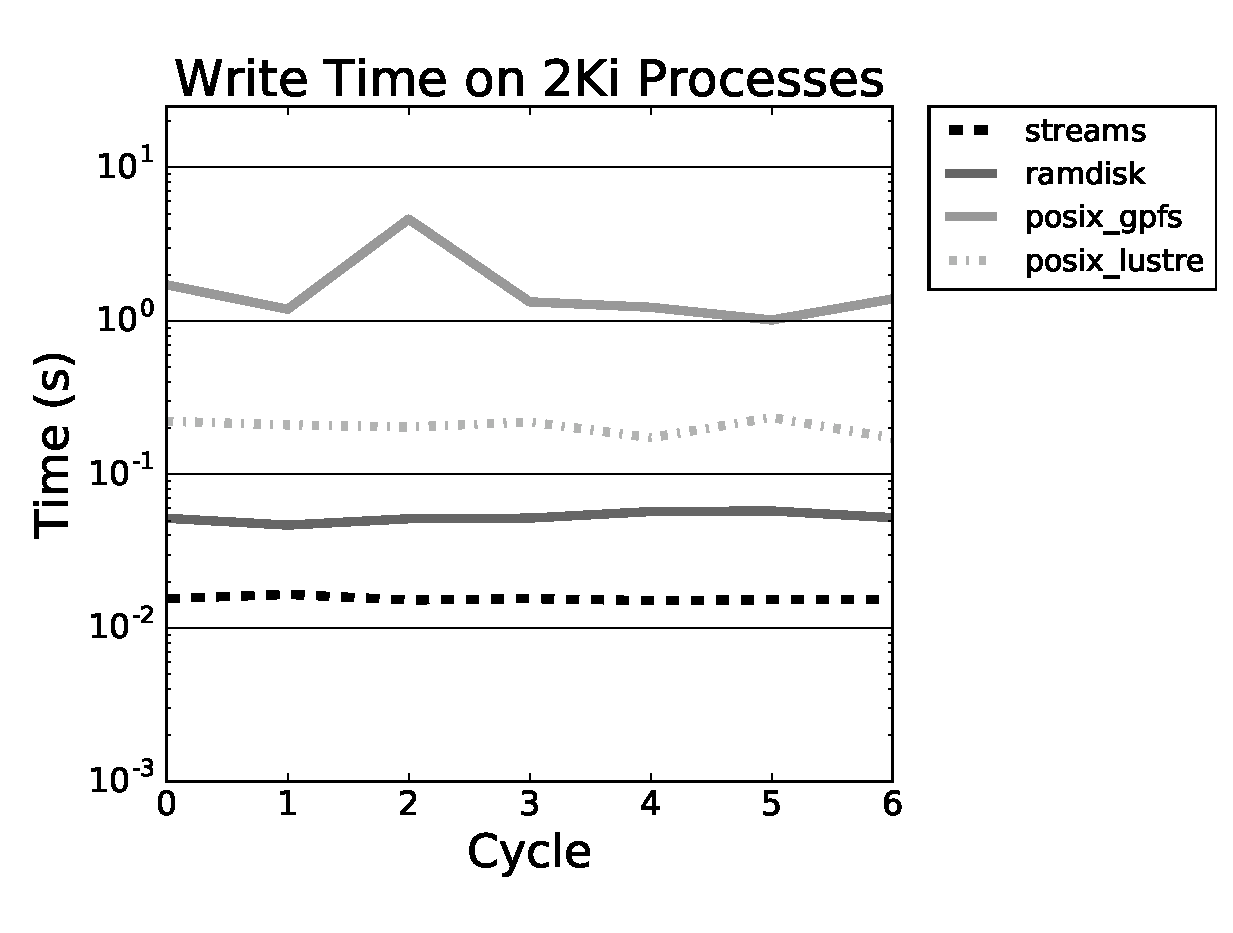
\includegraphics[width=.49\textwidth]{results/phasta-dambreak/theta/chef2048write.eps}
    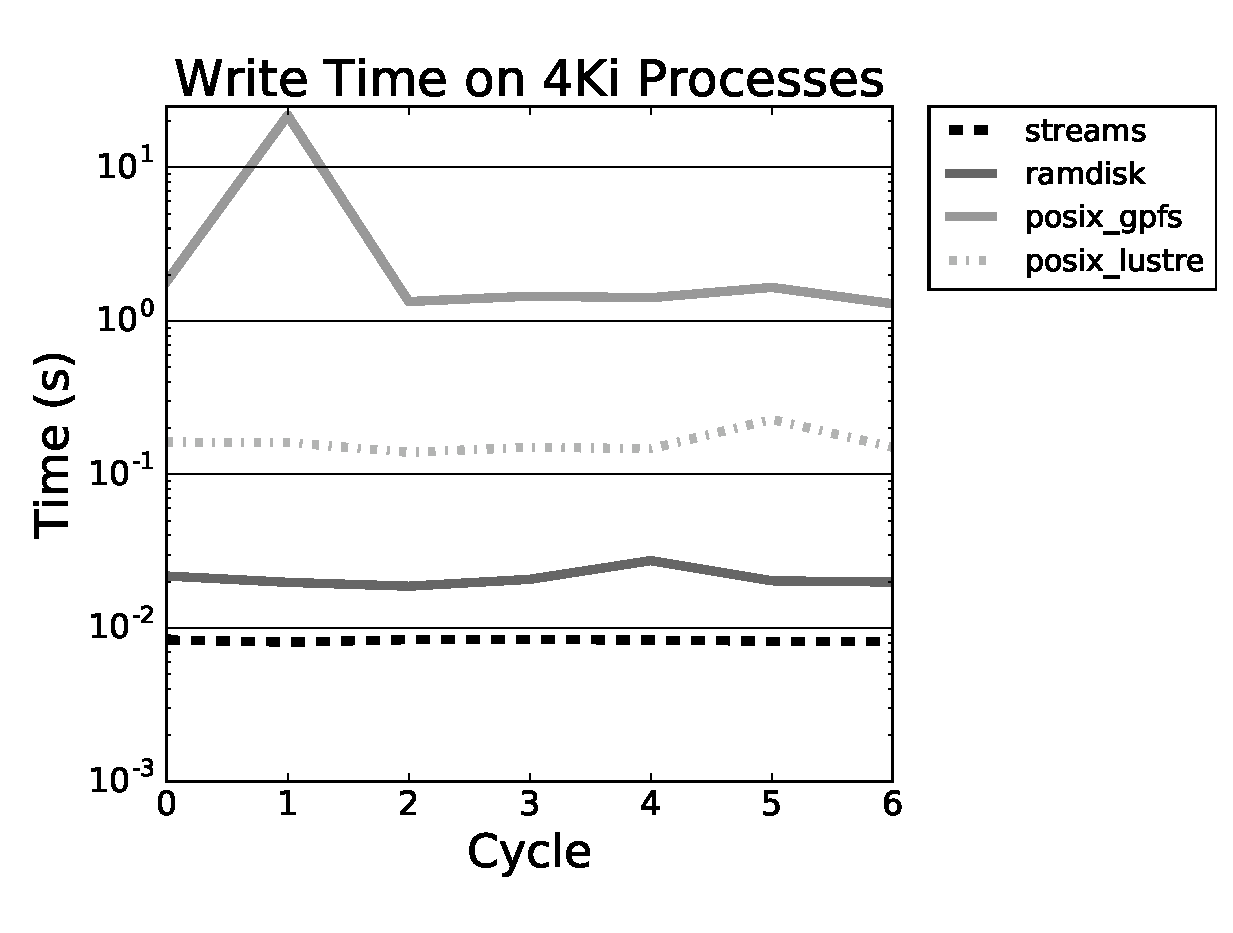
\includegraphics[width=.49\textwidth]{results/phasta-dambreak/theta/chef4096write.eps}
    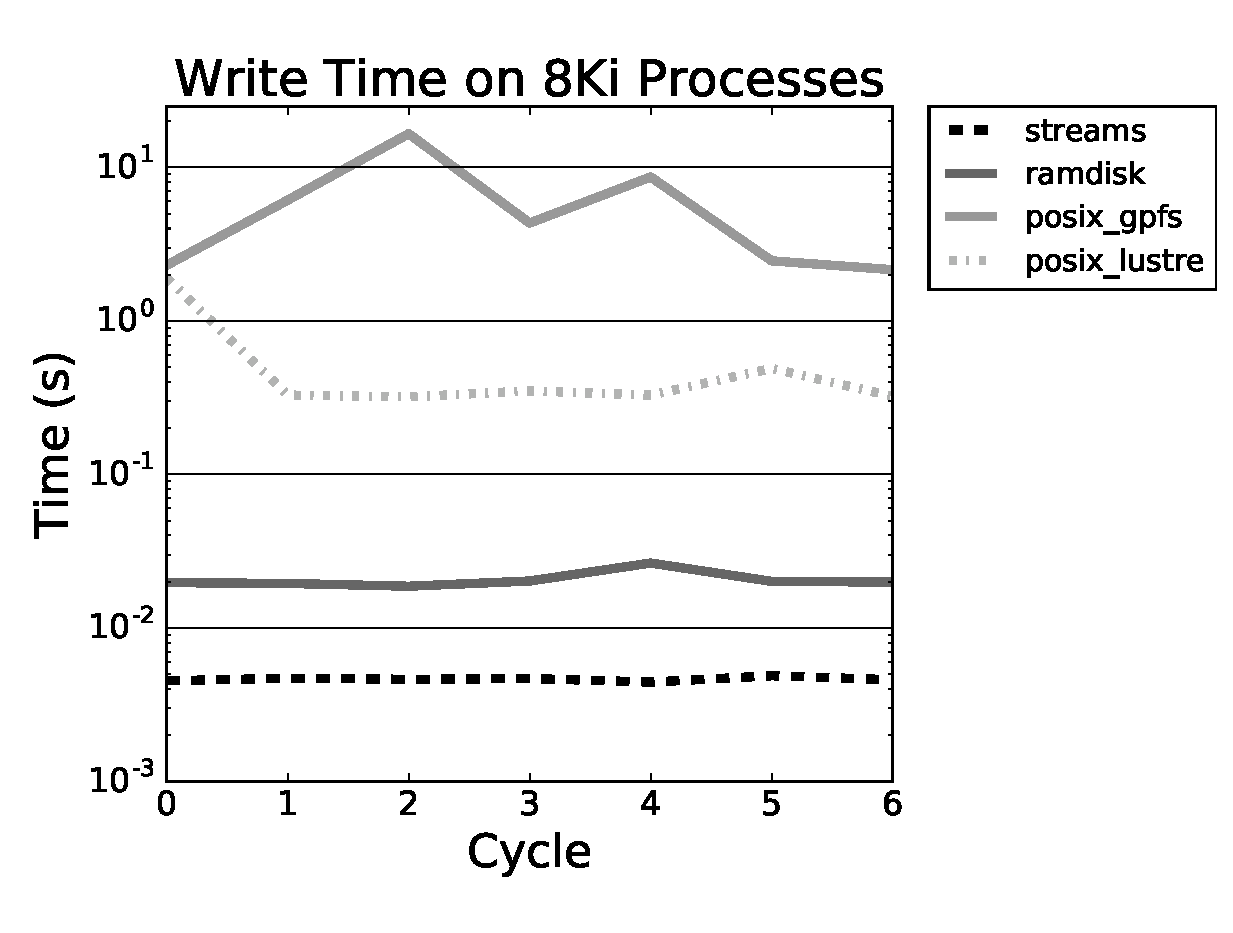
\includegraphics[width=.49\textwidth]{results/phasta-dambreak/theta/chef8192write.eps}
    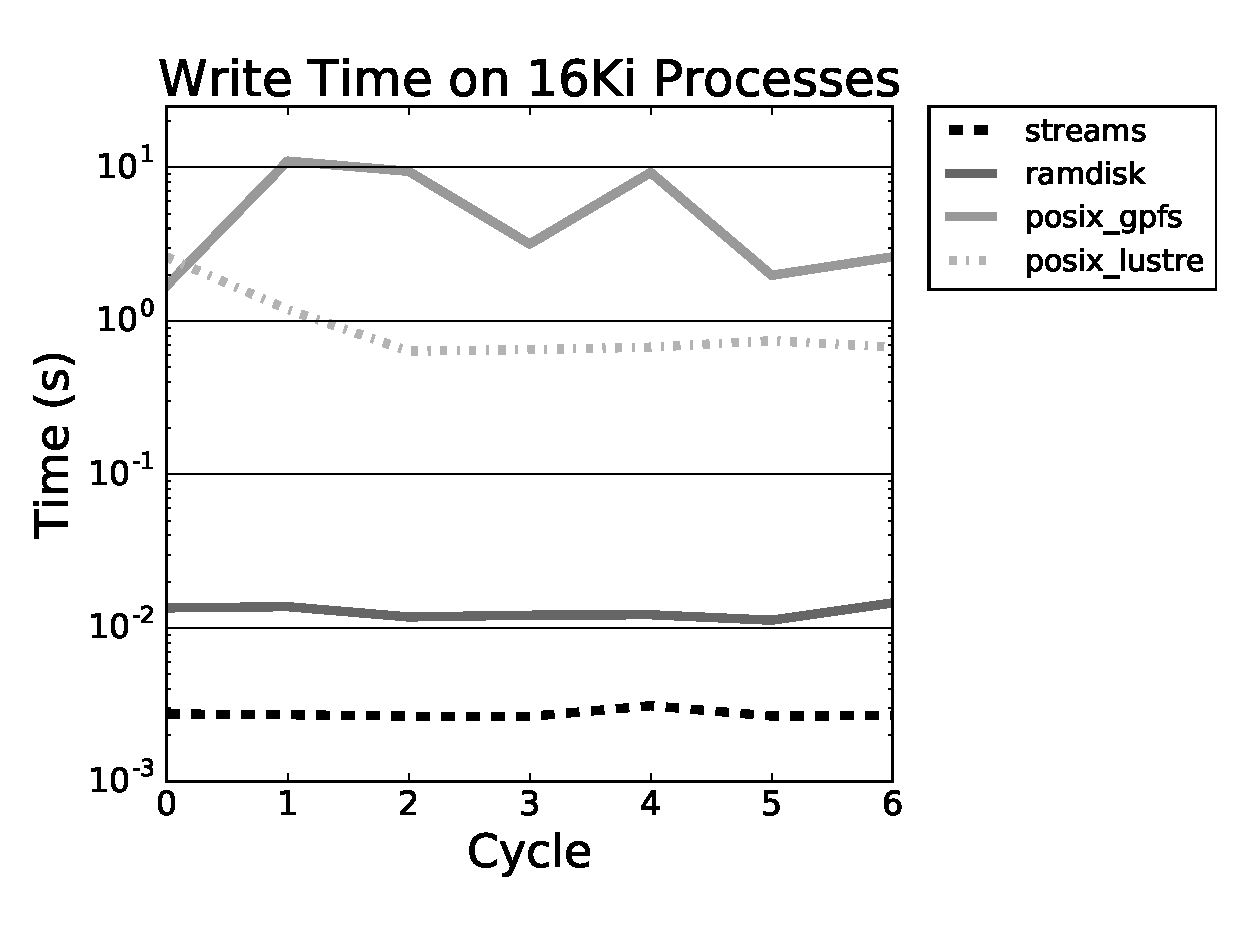
\includegraphics[width=.49\textwidth]{results/phasta-dambreak/theta/chef16384write.eps}
    \caption{chef write times.}
    \label{fig:chefwrite}
  \end{subfigure}
  \caption{
    Time for chef to read and write using streams, ramdisk, and POSIX on ALCF
    Theta.  Lower is better.
  }
  \label{fig:cheftimes}
\end{figure}

Across all process counts read and write times are highest when using
POSIX files on the GPFS filesystem.
The Lustre filesystem performs better, especially for writes, and has
significantly lowered variability between cycles.
As expected though, Lustre is slower than the ramdisk and streams.
Stream writes and reads outperform Lustre by over an order of magnitude at all
process counts.
At 8Ki and 16Ki the performance gap widens to over two orders of magnitude.
Also, note that the stream and ramdisk performance improves with the increase in
process count and reduction in per process transfers (see
Fig.~\ref{fig:totalBytes}), whereas the filesystem performance degrades for
Lustre and remains flat for GPFS.
Clearly, avoiding operations accessing the shared file system can save a
significant amount of time over the course of a parallel adaptive analysis.

Furthermore, serial testing on one Theta node indicates that using preallocated
buffers with \texttt{open\_memstream} can further improve streaming write
performance by over two times.
The performance penalty of dynamic buffer expansion for the non-preallocated
writes can clearly be seen in Fig.~\ref{fig:prealloc} by the large drop in
effective (bytes/time(open+write+close)) bandwidth at approximately 0.25MB, 0.5MB,
1MB and 2MB.
Likewise, POSIX file performance may be improved through use of the POSIX
asynchronous I/O interface (\texttt{aio})~\cite{bhattacharya2003asynchronous},
but we have not tested these APIs on Theta.

\begin{figure} \centering
  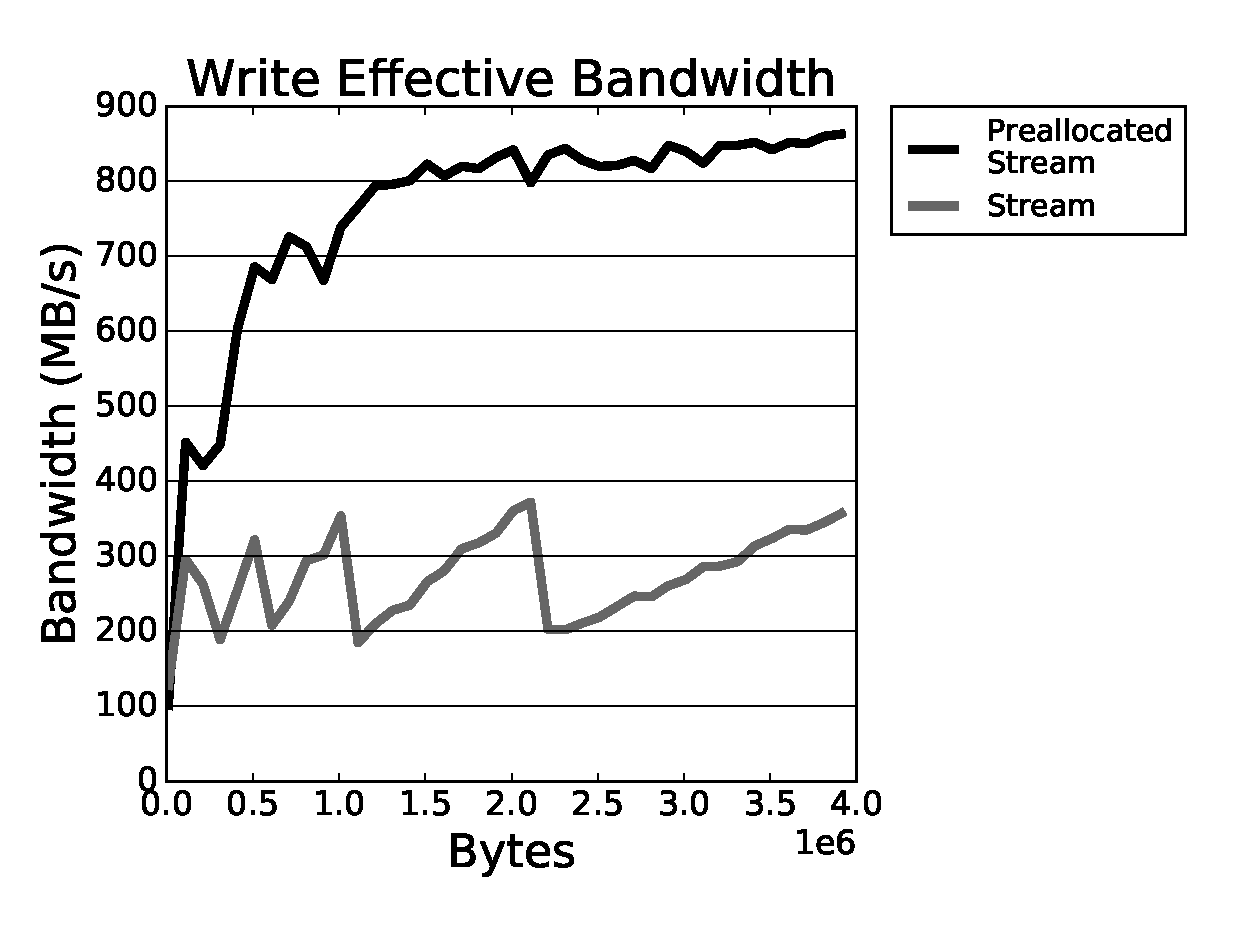
\includegraphics[width=.55\textwidth]{results/streamPrealloc/streamPreallocWriteEffectiveBandwidth.eps}
  \caption{
    Streaming write performance with and without preallocation on a single node
    of ALCF Theta in the cache-quad configuration.
    Higher is better.
    The code used for these tests is described in the Appendix.
  }
  \label{fig:prealloc}
\end{figure}
